%\section{The CMS Experiment}

The Compact Muon Solenoid (CMS) detector is a general purpose particle detector designed to investigate various physical phenomena concerning the SM and beyond it, such as Supersymmetry \cite{What_is_SUSY} ,
 Extra Dimensions and Dark Matter \cite{What_is_DM} . As its name implies, the detector is a solenoid which is  constructed around a superconducting magnet capable of producing a magnetic field of 3.8 T. The magnetic coil is 13m long with an inner diameter of 6m, making it the largest superconducting magnet ever constructed. The CMS detector itself is 21m long with a diameter of 15m and it has a weight of approximately 14,000 tons. The CMS experiment is one of the largest scientific collaborations in the history of mankind with over 4,000 participants from 42 countries and 182 institutions. CMS is located at one of these points and it essentially acts as a giant super highspeed camera that makes 3D images of the collisions that are produced at a rate of 40 MHz (40 million times per second). The detector has an onion-like structure to capture all the particles that are produced in these high energy collisions most of them being unstable and decaying further to stable particles that are detected.  CMS detector was designed with the following features (as shown in \autoref{CMSLayout}) :

\begin{enumerate}
	\item{A \textbf{magnet} with large bending power and high performance muon detector for good muon
identification and momentum resolution over a wide range of momenta and angles.}

	\item{An \textbf{inner tracking system} capable of high reconstruction efficiency and momentum resolution
requiring \textbf{pixel detectors} close to the interaction region.}

	\item{An \textbf{electromagnetic calorimeter} able to provide good electromagnetic energy resolution and  
a high isolation efficiency for photons and leptons.}

	\item{A \textbf{hadron calorimeter} capable of providing precise missing-transverse-energy and dijet-mass  
resolution.}

\end{enumerate}

\begin{figure}
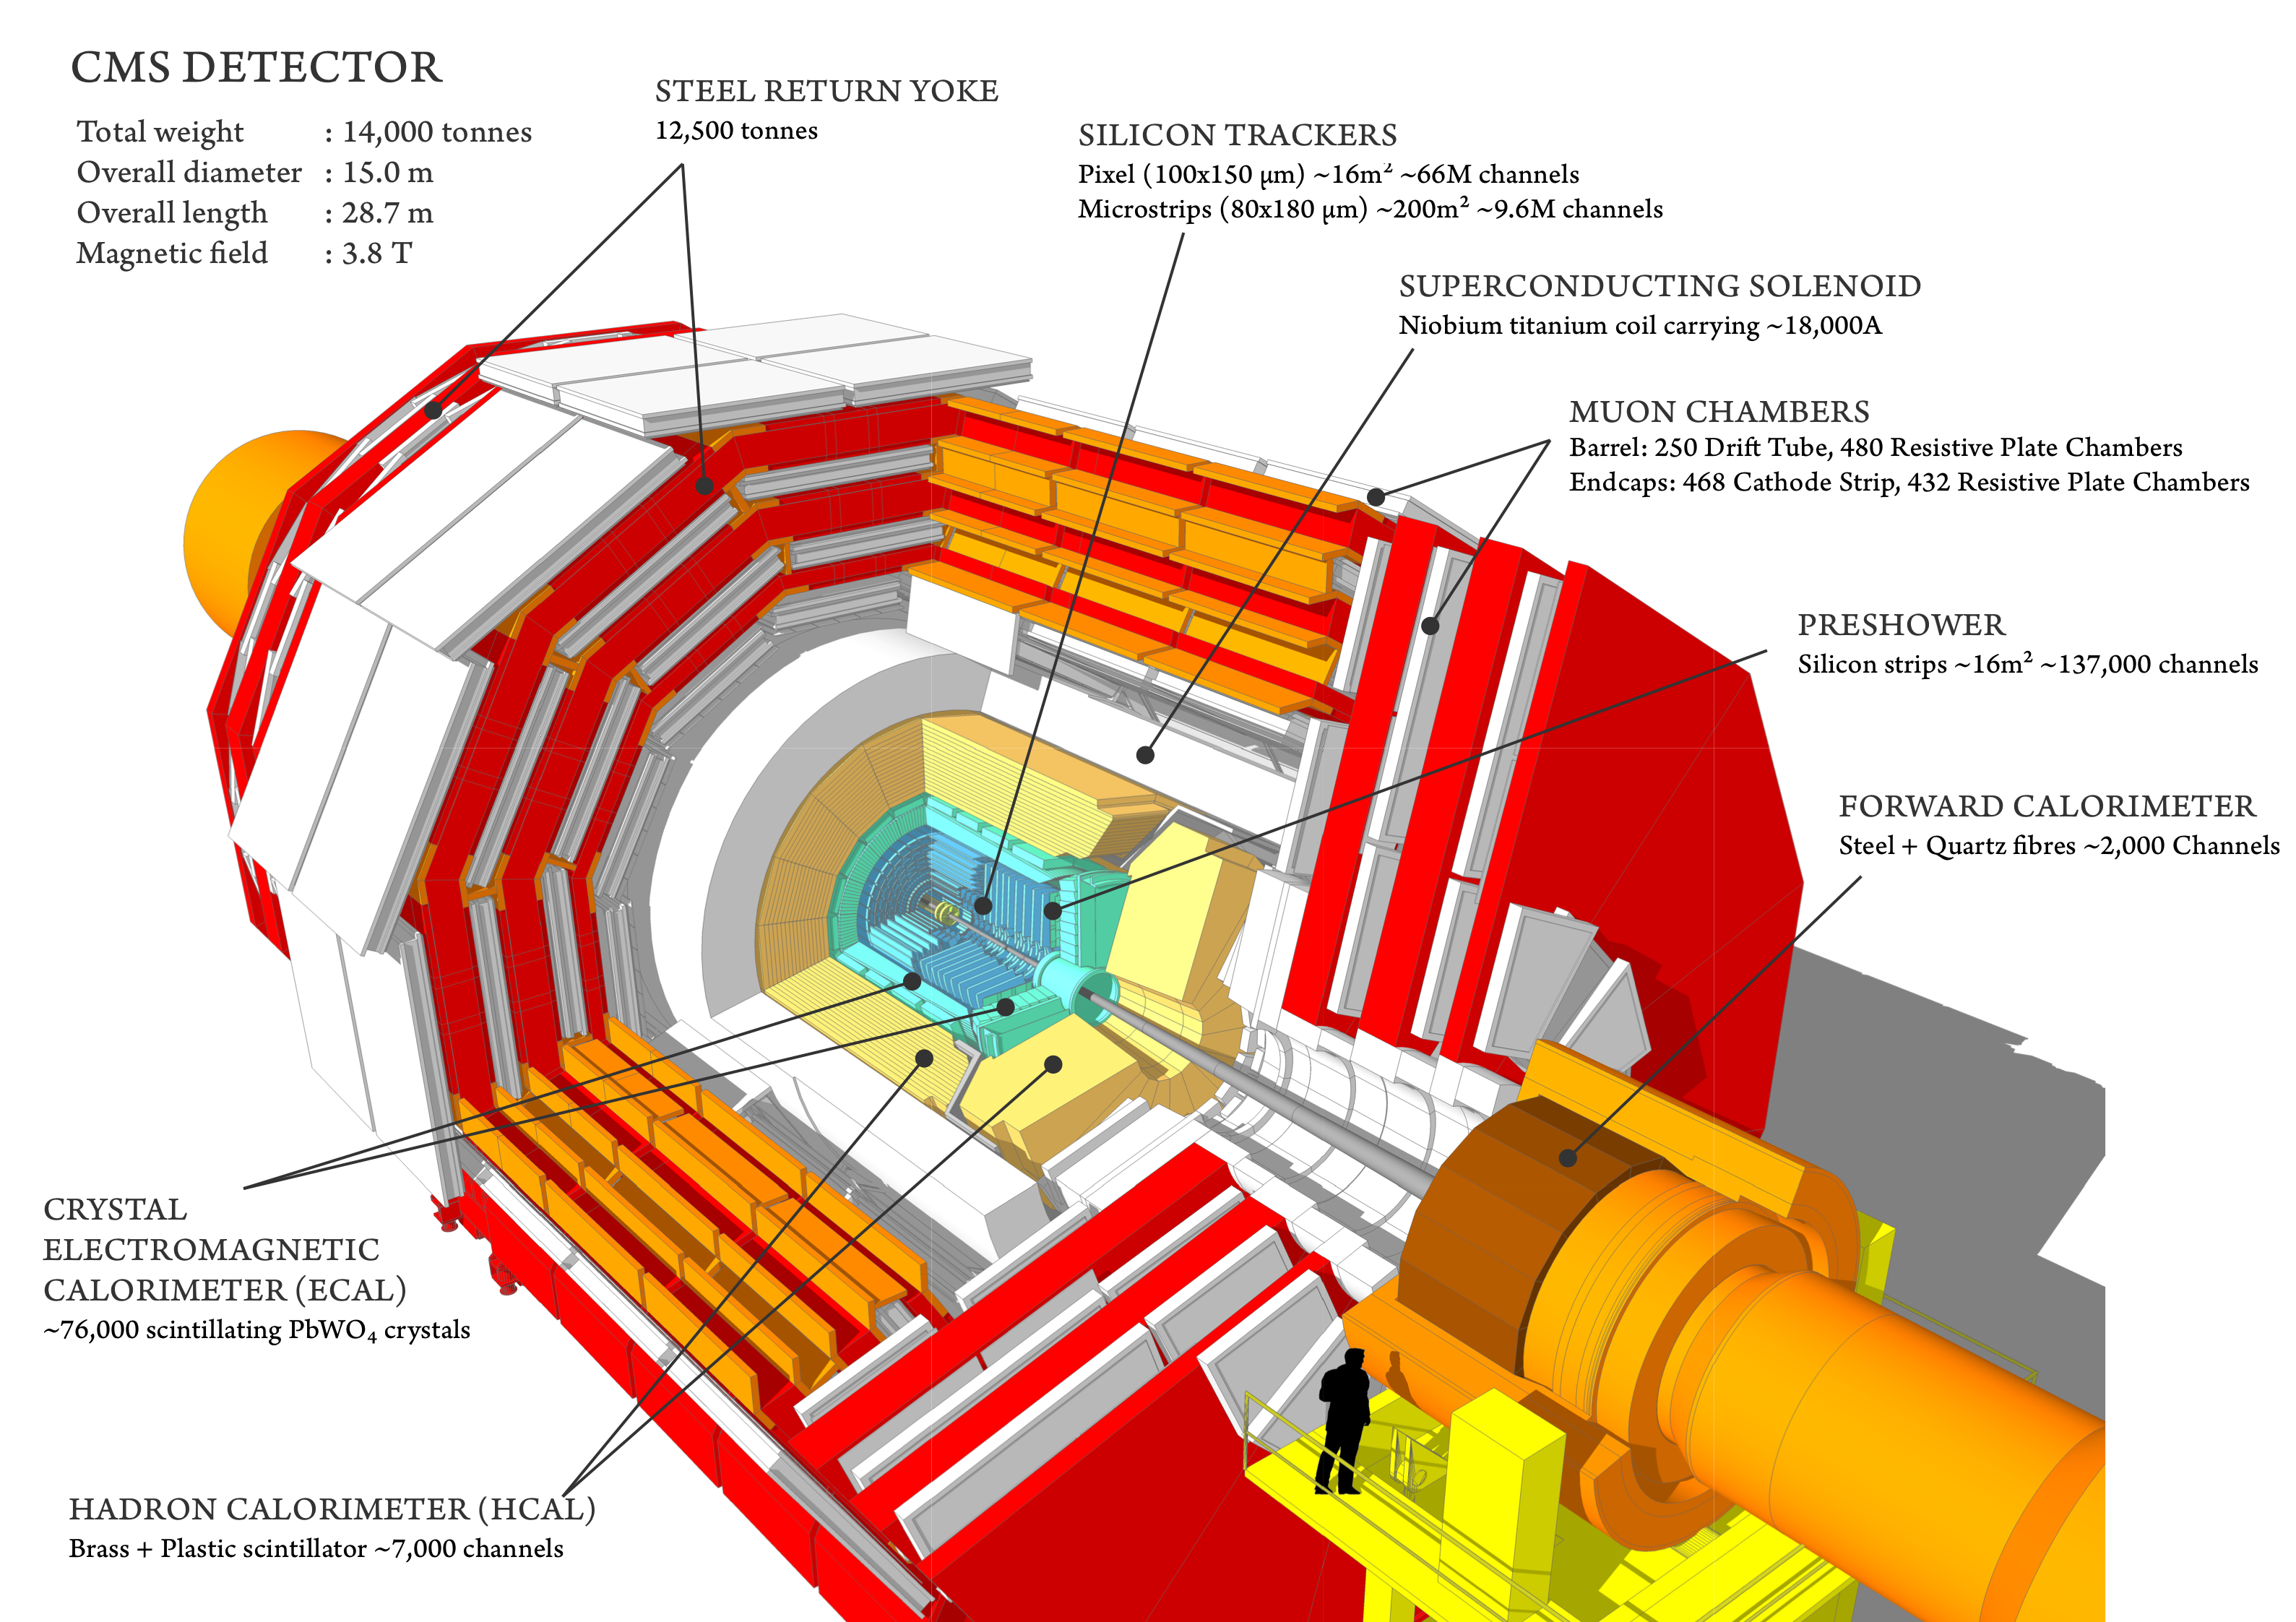
\includegraphics[width=\linewidth]{CMSLayout.png}
\caption{CMS Detector \label{CMSLayout}}
\end{figure}

\cite{CMS_detector} A property from these particles that is exploited is their charge. Normally, particles produced in collisions travel in a straight line, but in the presence of a magnetic field, their paths are skewed and curved. Except the muon system, the rest of the sub-detectors lie inside a 3.8 Tesla magnetic field . Due to the magnetic field the trajectory of charged particle produced in the collisions gets curved  (as shown in \autoref{CMSLayers} ) and one can calculate the particle's momentum and know the type of charge on the particle.  The Tracking devices are responsible for drawing the trajectory of the particles by using a computer program that reconstructs the path by using electrical signals that are left by the particle as they move.  The Calorimeters measure the energy of particles that pass through them by absorbing their energy with the intent of stopping them. The particle identification detectors work by detecting radiation emitted by charged particles and using this information they can measure the speed, momentum, and mass of a particle. After the information is put together to make the “snapshot” of the collision one looks for results that do not fit the current theories or models in order to look for new physics.

\begin{figure}[h]
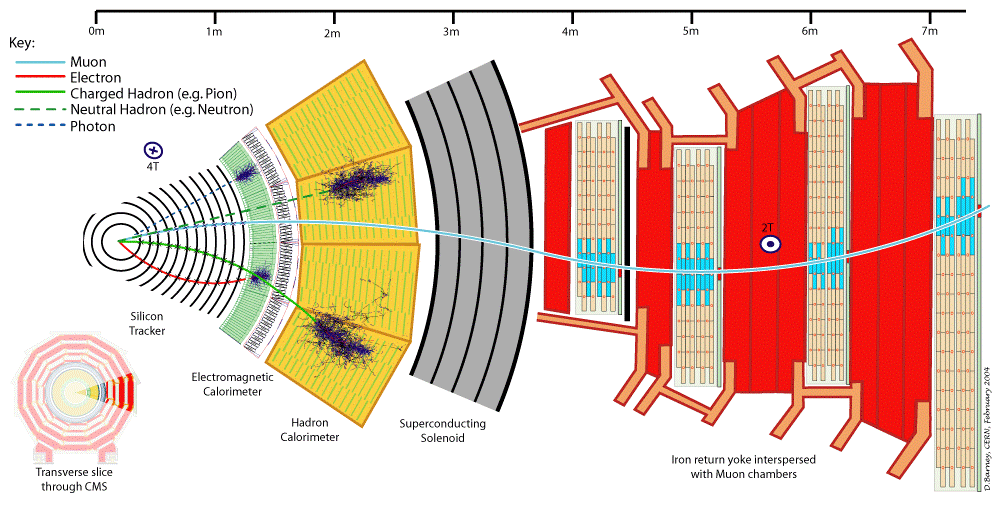
\includegraphics[width=.90\linewidth]{CMSLayers.PNG}
\caption{The trajectory of a particle traveling through the layers of the detector leaving behind it's signature footprint\label{CMSLayers}}
\end{figure}


The project focusses specifically on data collected from one of the Calorimeters, - the Hadron Calorimeter (HCAL). The HCAL, as its name indicates, is designed to detect and measure the energy of hadrons or, particles that are composed of quarks and gluons, like protons and neutrons. Additionally, it provides an indirect measurement of the presence of non-interacting, uncharged particles such as neutrinos (missing energy) . Measuring these particles is important as they can tell us if new particles such as the Higgs boson or supersymmetric particles (much heavier versions of the standard particles we know) have been formed. The layers of the HCAL are structured in a staggered fashion to prevent any gaps that a particle might pass through undetected. There are two main parts: the barrel and the end caps. There are 36 barrel wedges that form the last layer of the detector inside the magnet coil, there is another layer outside this, and on the endcaps, there are another 36 wedges to detect particles that come out at shallow angles with respect to the beam line.


